\chapter{Introduction} \label{chap:introduction}

\begin{abstract}
    Nuclear energy is at the core of world's sustainable development efforts and poised to take on an even bigger role as the world collectively moves to decarbonise many sectors of the economy. Despite its potential, several challenges remain and are related to sustainability, reliability, economic competitiveness, safety, risk of proliferation and anticipated future needs beyond electricity \cite{GIF:2009aa}. Several advanced reactors, like \gls{msr}, are being developed to overcome these challenges but such reactors pose unique challenges in terms of engineering design, modelling and construction of these reactors. The design issues are themselves quite complicated and span a wide array of knowledge domains such reactor physics, chemistry, materials science, fluid flow and heat transfer, etc. To address these challenges, modelling and simulation and  high-performance computing resources are being heavily leveraged. This is driving the development of advanced simulation tools such as those being developed under the \gls{neams} program.
    
    This work aims to support and augment the material modelling capabilities developed under \gls{neams} by adding capabilities which, until now, had been missing from the \gls{neams} code suite. This chapter aims to give the context to the work by describing the challenges faced in nuclear material design, the effect of thermochemistry and how modelling and simulation is key to tackling the challenges. This is followed by a description of the \gls{moose} framework which this work contributes to through the development of a new code called {\GEM} which has also been introduced. The developed code is applicable to all reactor technologies but the main thrust was \gls{msr} so the discussion will be in that context.
\end{abstract}

%==============================================================================================================================
%												Challenges in Nuclear Material Design
%==============================================================================================================================	
\section{Material Challenges in Nuclear Systems}
	Design and discovery of materials most suited for a specific application is an intrinsic part of development of new technology as many engineering designs can only be as good as the materials available during design and innovation. In conventional materials, the mechanical, thermophysical and chemical properties are often of main interest but nuclear materials must overcome significant challenges to provide the desired levels of reliability and safety commensurate to strict quality assurance requirements. Nuclear reactors present extreme environments for components irrespective of the reactor technology and not only do materials need to meet the physical and chemical performance requirements, but must also demonstrate desirable nuclear physics characteristics. The core in particular presents an exceptionally harsh environment of high temperature, high pressure, high stresses, intense radiation and a chemically aggressive environment and the properties desirable from a nuclear perspective, such as high power density, exert high operational burdens on fuels and structural materials \cite{Zinkle:2013aa}.  As advanced reactor designs gain increasing traction, the material-challenges are only going to get worse. Advanced reactors, such as \gls{msr}, operate not only at higher temperature, pressure and irradiation flux but also with coolants that present more challenging corrosion problems than the current lot of \gls{lwr} and \gls{hwr} \cite{Allen:2010aa}. Moreover, Generation {IV}  reactors are expected to have a longer operating time of at least sixty years.
 
%==============================================================================================================================
%														Thermochemistry
%==============================================================================================================================	
% \section{Thermochemistry in Nuclear Systems}
    Thermochemistry and principles of computational thermodynamics play a key role in nuclear material modelling. Since nuclear materials are continuously evolving due to transmutations, fission product generation and decay, so do their material properties. The laws of thermodynamics govern many phenomena in nuclear materials and are important for applications such as understanding phase equilibria, which affects nucleation and dissolution of phases, oxidation potential of cladding, thermochemical properties of fuels and many others. As such, thermodynamic principles are sufficient for predicting many phenomena and are, at a minimum, imperative to understanding more complex and dynamic physics. Some of the key applications of thermodynamics that make it indispensable to \gls{msr} design and development process include but are not limited to:
    \begin{enumerate} \compresslist
        \item Optimising fuel salt composition and prediction of thermal stability of fuel and structural materials materials.
	\item Understanding fission product chemistry and their effect on material properties.
	\item Predicting chemical interactions between fuel and structural materials.
	\item Predicting impact of impurities on molten salt corrosion in \gls{msr}.
        \item Source term analyses and predicting phases that form between reactor materials under severe accident scenarios.
    \end{enumerate}
	
	While the concepts of thermodynamics can be embodied in both non-equilibrium and equilibrium descriptions, it is often thermodynamic equilibrium that is leveraged in applications. Even when the materials are, in many cases, in non-equilibrium conditions, an understanding of the phases that shall form under equilibrium conditions provides valuable knowledge as it gives the direction of evolution of the system.  In fact, in nuclear materials, the high temperature conditions lead to a rapid approach to equilibrium and under suitable conditions, make equilibrium thermodynamics a suitable approximation.
	
%==============================================================================================================================
%													Modelling and Simulation
%==============================================================================================================================	
\section{Modelling and Simulation}
	The traditional approach to studying materials was almost entirely experimental but recent developments in modelling and high performance computing have resulted in a much stronger collaboration and integration among theory, experiments and computational science \cite{STAN200920}. Multiscale, multiphysics models and simulations enable investigations over a wide range of length and time scales which would otherwise be unfeasible using only experiments. Thus, computational models help augment and guide experimental campaigns and support economical discovery and design of materials within reasonable lead times.

	Complex interactions between the different physical phenomena occurring in the materials are often very tightly coupled and many important aspects are inherently multidimensional  as well \cite{WILLIAMSON2012149}. As an example, one can consider \gls{msr} where, as shown in Figure~\ref{fig:msr_mf}, multiple physics  are required for understanding the behaviour and for predicting phenomena such as mass accountancy. Another aspect to consider is that of the different time and length-scales involved with length-scales ranging from inter-atomic spacing to meters, and time-scales ranging from microseconds to years. For example, radiation defects start within picoseconds at the atomistic scales and propagate to larger length-scales over time-scales which are several magnitudes longer.
	\begin{figure}[htb]
		\centering
		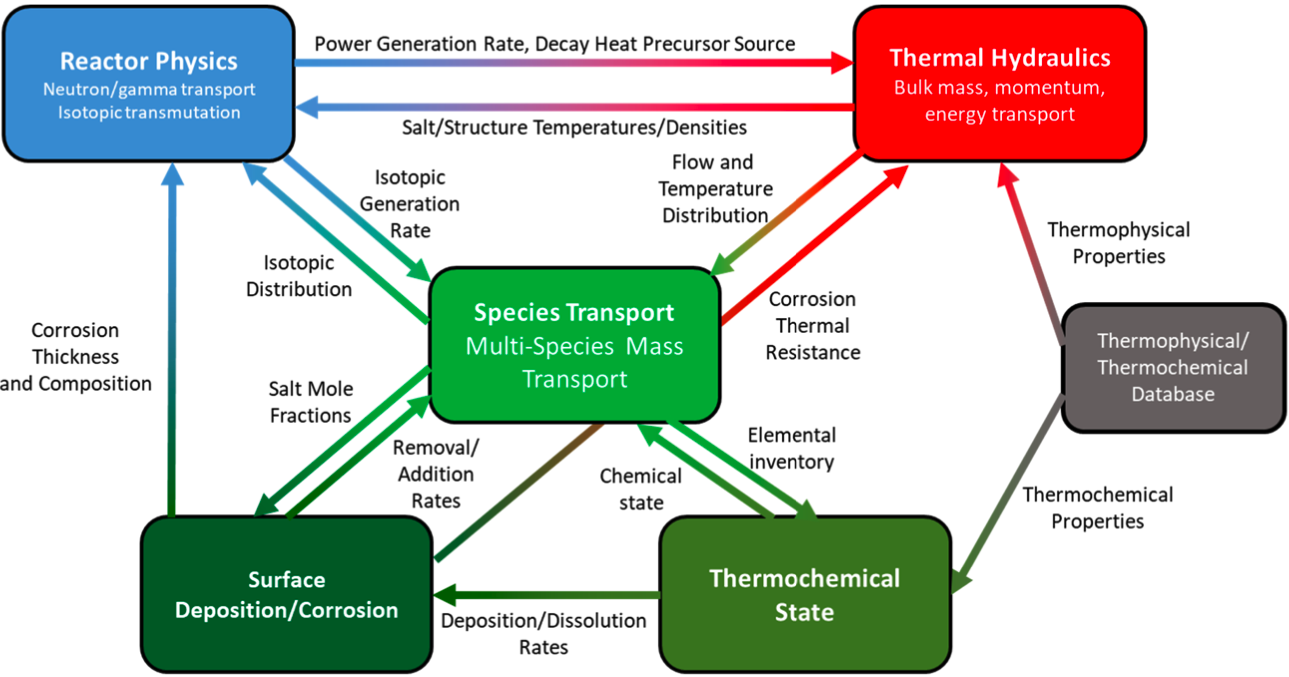
\includegraphics[width=0.75\textwidth]{figures/chapter-1/MSR_MP}
		\caption[Multiphysics phenomena in \glsxtrfull{msr}.]{Multiphysics phenomena in \glsxtrfull{msr} \cite{McMurray:2021aa}.}
		\label{fig:msr_mf}
	\end{figure}
	
	 Evidently, modelling and simulation of nuclear materials requires a multiscale, multiphysics approach. However, such simulations have been decently challenging until recently and with significant limitations on the amount of computational resources available even a couple of decades ago, a majority of modelling and simulation efforts adopted an operator-splitting approach based on Picard iterations. Such simulations usually focused on only the engineering scale behaviour and usually relied on continuum or bulk description of the phenomena. In doing so, experimental observations and operational experience were relied on for the validity of results and often very conservative safety margins were added to design parameters. As an example, nuclear fuel behaviour has been modelled as a solid mechanics problem coupled with conductive heat transfer and fission gas release wherein the material properties are often either assumed to be constant or described using simplified models based on empirical correlations. Though these methods were suitable for previous and current generation of nuclear reactors, addressing the materials challenges for advanced reactors is usually beyond their capability. In fact, there has been an increasing impetus on leveraging lower scale information to inform models on larger scales and solving the governing equations as a system rather than as individual problems.  Since such an approach is rooted in fundamental principles, the transfer of information between scales, through characteristic parameters such as density, energy, temperature, etc., results in a much more accurate description of material behaviour \cite{STAN200920}. The numerous modelling and simulation tools available at different length and time scales are shown in Figure~\ref{fig:multiphys}.
	\begin{figure}[htb]
		\centering
		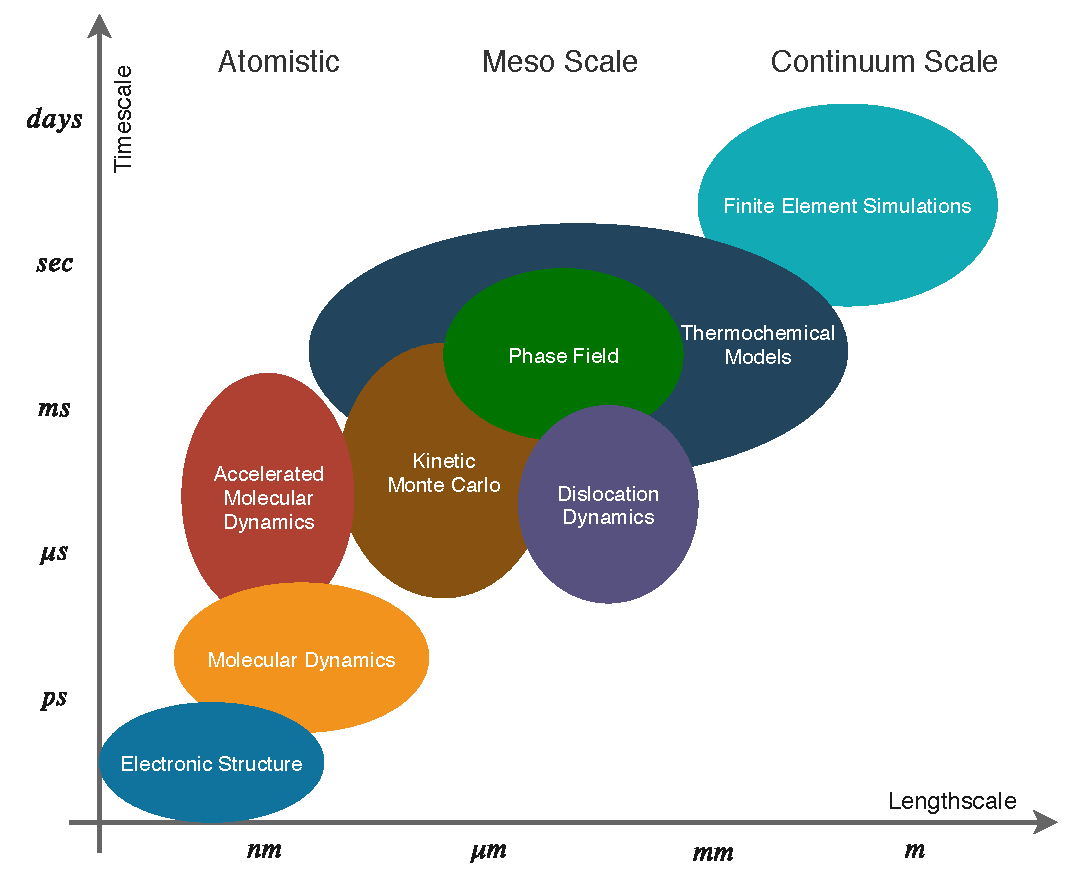
\includegraphics[width=0.75\textwidth]{figures/chapter-1/Multiphysics.pdf}
		\caption[Multiscale methods used for materials modelling simulation]{Multiscale theoretical and computational methods used for materials model development and computer simulation \cite{STAN200920}.}
		\label{fig:multiphys}
	\end{figure}
	
\subsection{Computational Thermodynamics}
    The modelling and simulation tool that is of particular relevance to this work is computational thermodynamics. Phase and chemical behaviour of nuclear materials is governed by the thermochemical equilibrium state. Computational thermodynamics is an essential tool for calculating both phase equilibria and thermodynamic properties of the system. It is rooted in the \emph{\gls{calphad}} approach shown in Figure~\ref{fig:calphad}. \gls{calphad} combines experimental and theoretical information and tunes parametric models to describe thermodynamic properties of materials like Gibbs energy, enthalpy, heat capacity, etc. \cite{Lukas07}.
	\begin{figure}[htb]
		\centering
		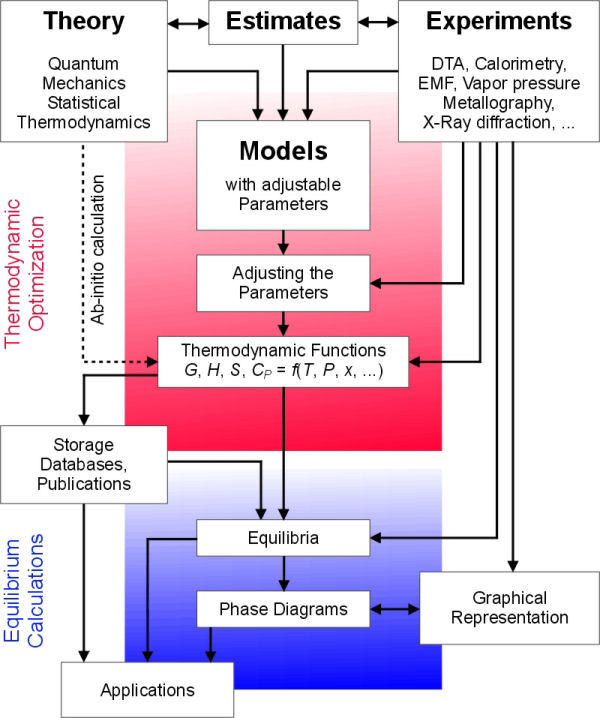
\includegraphics[width=0.6\textwidth]{figures/chapter-1/Calphad_method}
		\caption[Principle of CALPHAD method]{Principle of \gls{calphad} method by Zinkevich \cite{Zinkevich:2003aa}.}
		\label{fig:calphad}
	\end{figure}

	Capturing thermodynamic equilibria in multiphysics codes has traditionally relied on empirical correlations and the interest in direct coupling of thermodynamic equilibrium codes with multiphysics model is only a recent trend. While the empirical correlations do not convey the high fidelity of full thermodynamic analysis, performing thermodynamic equilibrium analysis within multiphysics codes is normally a very complex process and can significantly impede the computational performance of such codes. However, the recent developments in high performance computing have facilitated the use of equilibrium thermodynamics in multiphysics  simulations and it is enabling the study of many phenomena which until now were not well understood.
	
	The inputs and outputs of thermodynamic equilibrium calculations are shown in Figure~\ref{fig:Thermod}. While, other physical conditions are possible, e.g. isochoric processes, the discussion here is restricted to isothermal, isobaric conditions. The Gibbs energy functions are available in many databases, such as \gls{mstdb} and \gls{taf-id}, which are developed experimentally using the \gls{calphad} method described above and atomistic calculations are often used to inform and fill in the knowledge gaps where experiments might not be possible. The results from equilibrium calculations include the stable phases, speciation of the phases, and thermodynamic properties like Gibbs energy, chemical potentials, heat capacities, etc.
	\begin{figure}[ht]
        		\centering
        		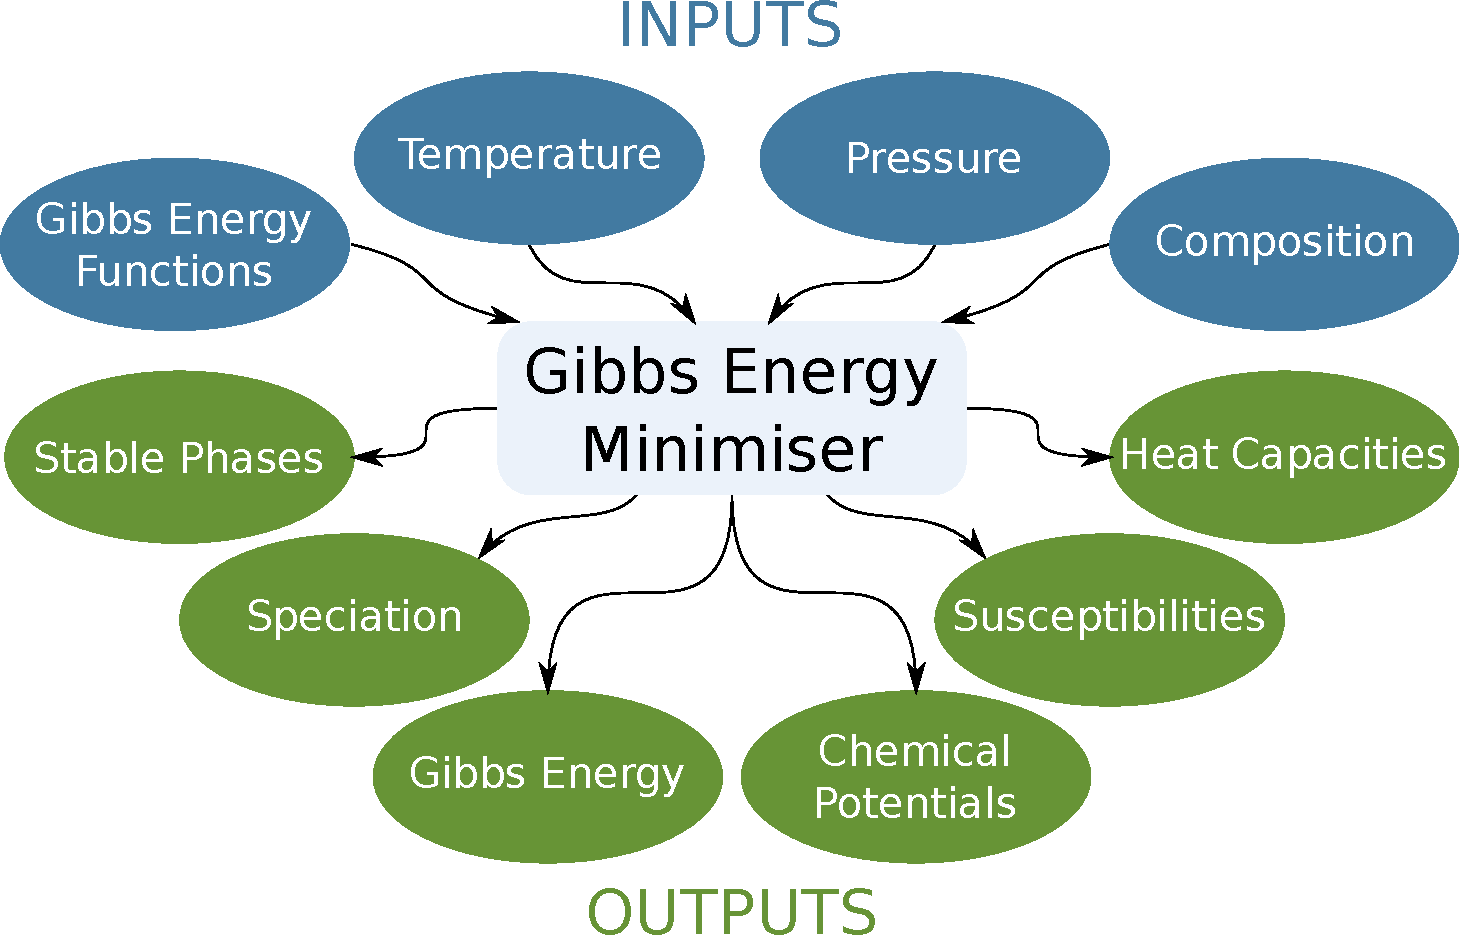
\includegraphics[width=0.75\textwidth]{figures/chapter-1/thermodynamics.pdf}
        		\caption{Input and output parameters of thermodynamic equilibrium calculations.}
        		\label{fig:Thermod}
    	\end{figure}
	
\subsection{Multiphysics Object Oriented Simulation Environment}
	The \glsxtrfull{moose} is a simulation framework that has been developed with the aim of harnessing modern massively parallel computing resources to perform complex multiphysics simulations. The goal of \gls{moose} is to provide simplified interfaces for user facing tasks such as specification of partial differential equations, boundary conditions, material properties and all aspects of a simulation while handling complex background tasks such as parallel, adaptive, nonlinear, finite element solve internally \cite{Permann:2020aa}. Originally created at the Idaho National Laboratory in the United States, \gls{moose} is open-source framework which leverages state-of-the-art libMesh code \cite{Kirk:2006aa} for finite elements and the \gls{petsc} \cite{Balay:2022ab,Balay:2022aa} for leading-edge numerical methods/solvers. \gls{moose} has been used to build multiple community-developed physics "modules" \cite{Guillaume:2021aa,Guillaume:2021ab,Adhikary:2016aa,Wilkins:2020aa,Shemon:2021aa} and several application libraries which are used by governments, industry and academia. 
	
	For nuclear reactor modelling, apart from the \gls{moose} modules, several export-controlled applications have been developed. These include {RELAP-7} \cite{Zhang:aa} for system level thermal hydraulics, {Rattlesnake} \cite{Wang:2021aa} for neutronics, etc. For nuclear material simulations, the {\gls{moose}} framework consists of two main applications the macroscale fuel performance code {Bison} \cite{WILLIAMSON2012149} and the mesoscale phase field code {Marmot}  \cite{Tonks12}. 
	
	Simulation of nuclear reactor fuel performance involves complex thermomechanical processes between fuel pellets, made of fissile material, and the protective cladding barrier that surrounds the pellets. {Bison} is an engineering scale code developed to predict the nuclear fuel performance under normal, off-normal, and accident conditions. By using highly efficient computational methods, it enables three dimensional, fully coupled multiphysics simulations on high fidelity geometric representations of fuel pins/pellets. {Bison} has been designed to be highly scalable and does not require the use of operator splitting, staggered or predictor-corrector approaches \cite{WILLIAMSON2012149}.

	Due to its simple concept and large range of applicability, the phase field approach is a popular and powerful tool to model microstructure and has been applied in problems such as grain boundary migrations, martinistic transformation, two-phase flow, etc. The phase field approach treats all material interfaces as diffuse by representing structural features with continuous variables which smoothly transition from one value to another. Thus, phase field method not only eliminates the need to explicitly discretise boundaries and interfaces, it also enables describing microstructure through a system of partial differential equations.  The {Marmot} phase field application has been developed to enable simulations of the microstructure evolution of nuclear fuels and materials under irradiation. By exploiting the object-oriented architecture of {\gls{moose}}, {Marmot} allows easy coupling of phase field with additional physics such as solid mechanics or heat conduction, to effectively predict the microstructural evolution at mesoscale. This allows prediction of evolution of material properties of nuclear materials under irradiation and can be used to inform engineering scale simulations and reduce the dependence of such simulations on empirical correlations. As a result, the multiscale framework can achieve true predictability even in compositional and operational regimes where little or no experimental data exists \cite{Tonks12}.

	Despite the wide ranging capability of \gls{moose}, there has been a lack of dedicated tools for modelling molten salt corrosion and to bridge this gap, a suite of tools have been developed under the \gls{neams} program of the United States Department of Energy. Corrosion is an electrochemical process composed of oxidation and reduction reactions, which are defined by the thermodynamics and kinetics of the system. While thermodynamics controls whether or not a material may corrode, kinetics influences how quickly the material will corrode. This corrosion behaviour is also significantly affected by the material microstructure and predicting corrosion therefore requires a multiphysics approach that can couple quantitative electrochemistry models of corrosion and chemical reactions with thermochemical equilibrium computations. Effectively, predicting corrosion and related phenomena like leaching and deposition requires a multiscale, multiphysics approach \cite{Mcmurray:2018aa}. The corrosion suite, shown in Figure~\ref{fig:yj_suite}, aims to couple atomistic and mesoscale modelling to thermochemical equilibrium calculations to create a unique corrosion modelling capability on the microstructural scale and use it to inform engineering scale codes aimed at solving species transport problem. At the core of the corrosion suite is the \gls{moose}-based application {\YJ} that couples quantitative models of corrosion with thermodynamic equilibrium and chemical kinetics models to predict the rate of material loss, corrosion product production and precipitate production in advanced nuclear reactors. 
	\begin{figure}[htb]
		\centering
		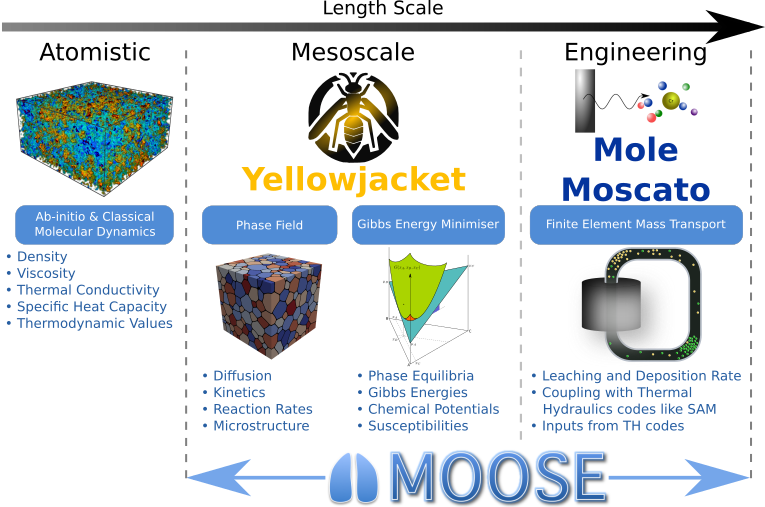
\includegraphics[width=0.95\textwidth]{figures/chapter-1/Yellowjacket_Suite.png}
		\caption[{\YJ} corrosion suite.]{{\YJ} corrosion suite. After McMurray et al. \cite{McMurray:2020aa}.}
		\label{fig:yj_suite}
	\end{figure}
 
  The software developed as part of this work adds native  equilibrium thermodynamic capability to \gls{moose} and its applications and is described in the following section.

%==============================================================================================================================
%															Molten Salt Corrosion
%==============================================================================================================================	
\subsection{Yellowjacket}
	Many emerging nuclear technologies, such as \gls{msr}, use high temperature fluids like molten fluoride/chloride salts, which can lead to the corrosion of salt-facing structural materials. Not only does corrosion impact the performance of structural materials with the possibility of compromising their integrity but it can also lead to other problems just as blocking of salt flow loops due to leaching from hot sections of the loop and deposition in the colder sections. In molten fluoride salts, the protective oxide layer on alloys typically relied upon for high-temperature corrosion resistance dissolves, thereby exposing the fresh alloy surface to the molten salt. In molten chloride salts, passivity has been observed; however, the oxide layer is prone to attack and may not provide the necessary corrosion protection \cite{Sridharan:2013aa}. The corrosion process is accelerated by the impurities present in the salt and enhanced further by the presence of dissimilar metals due to activity-driven corrosion. It has been observed the corrosion in molten salt is a microstructural phenomena with preferential leaching at grain boundaries as compared to bulk of the grain but there are significant gaps in the scientific understanding of the governing mechanisms such as the impact of impurities and irradiation \cite{Zheng:2018aa,Zhou:2020aa,Zhu:2021aa,Raiman:2018aa,Pillai:2021aa,Guo:2018aa}. {\YJ} relies on the phase field method for structural evolution and couples it with electrochemical descriptions, fracture models and thermochemical equilibrium solver to create a holistic environment for corrosion modelling and simulation \cite{Bhave:2022aa}.

	As shown in Figure~\ref{fig:yj_io}, {\YJ} phase field model requires several thermodynamic properties like Gibbs energies, chemical potentials and driving forces for the various phases which can be present in the system. This requires knowing the molar amounts of the different phases which would be present under given temperature, pressure and composition. However, at the interfaces, more than one phase can co-exist and the phase field models face a challenge in estimating the assemblage and thermodynamic properties. In such cases, a thermodynamic equilibrium solver can provide the required information to the phase field module. This is the prime driving force behind the development of {\GEM}. One may argue that the system will not be at equilibrium and that kinetics of the system will drive the corrosion behaviour and therefore might question the appropriateness of thermochemical equilibrium calculations. While the system is not really at equilibrium, it can be safely assumed that in the limiting case the system will be at equilibrium at any point in space and time.
	\begin{figure}[htb]
		\centering
		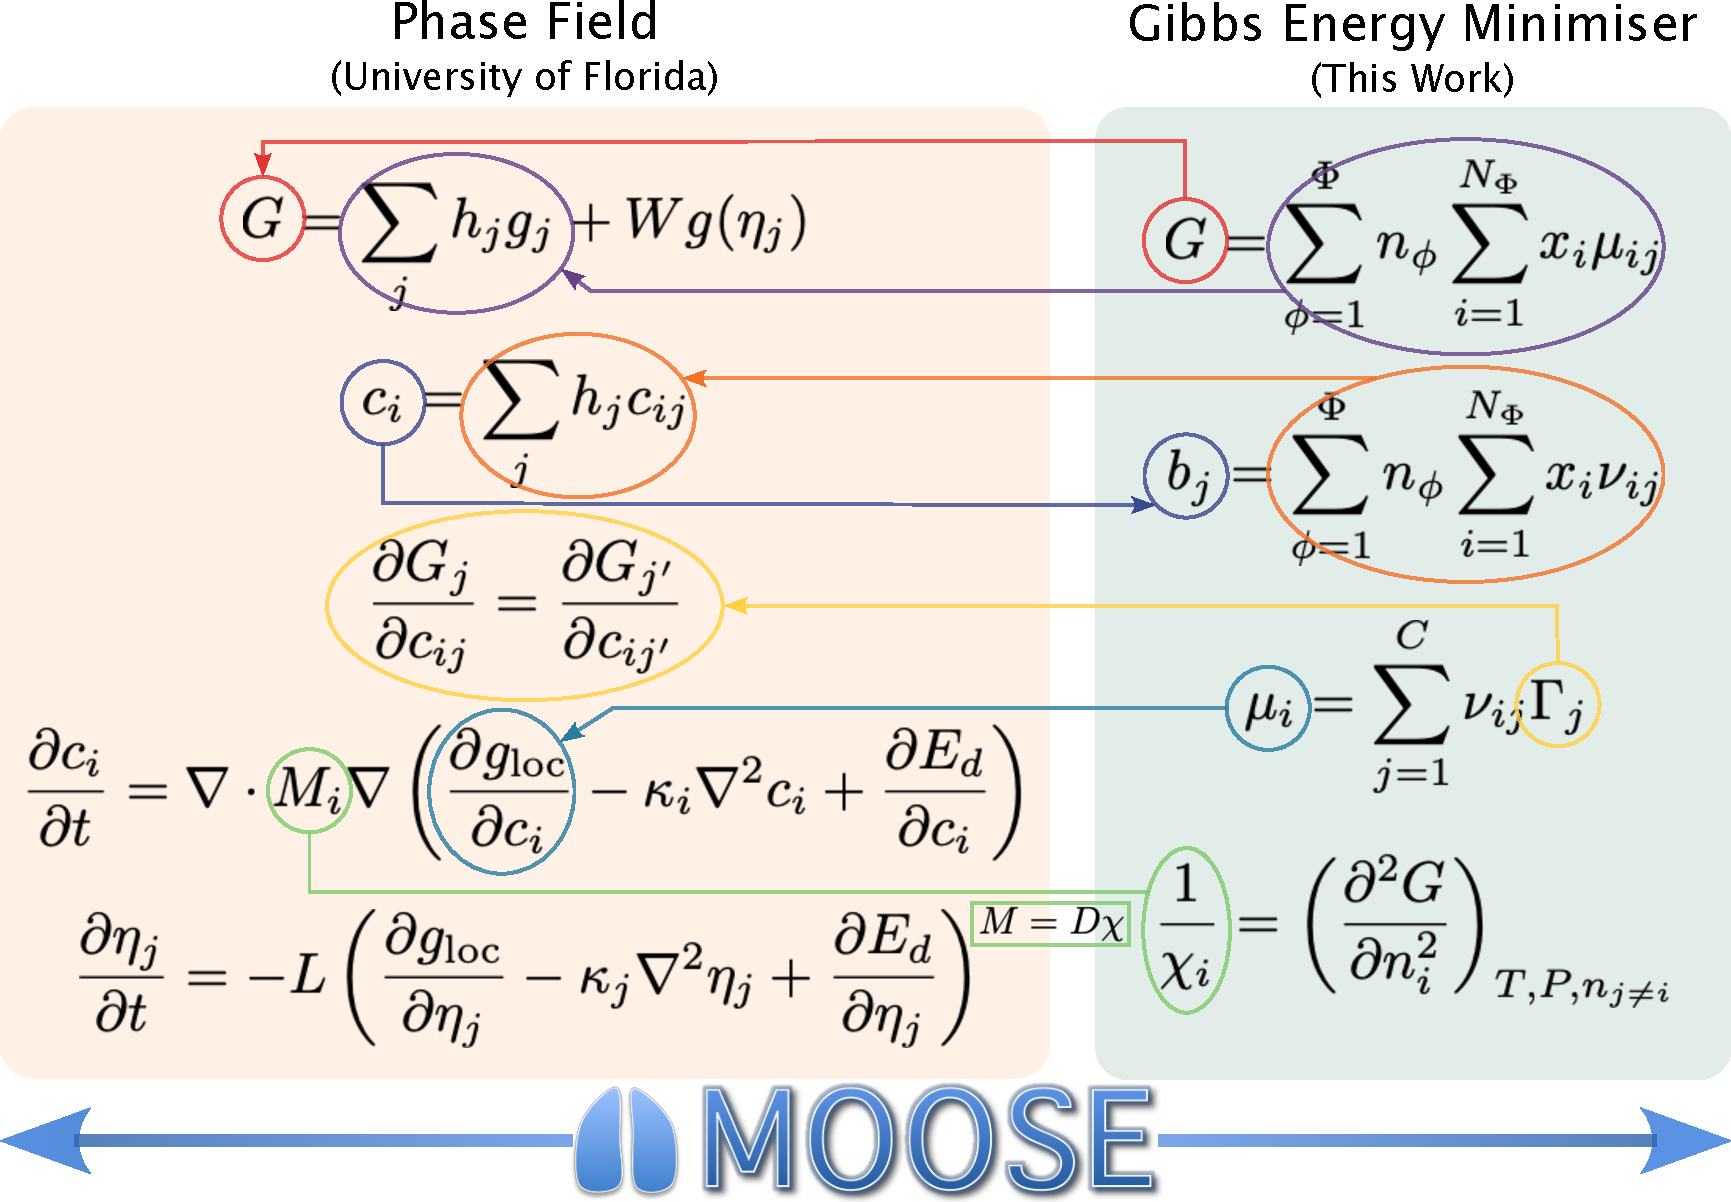
\includegraphics[width=0.8\textwidth]{figures/chapter-1/YJ_PF_IO.pdf}
		\caption{Information exchange between the phase field and equilibrium thermodynamics modules of \YJ.}
		\label{fig:yj_io}
	\end{figure} 	

	{\YJ} is multi-institutional collaborative effort between the Idaho National Laboratory, University of Florida, and Ontario Tech University.  In {\YJ}, the phase field module was implemented at University of Florida, computational thermodynamics development was performed as part of this PhD thesis at Ontario Tech University and \gls{moose}-integration was primarily done at Idaho National Laboratory. The main motivation behind this work was to enable direct coupling of thermodynamic equilibrium calculations in \gls{moose}-based multiphysics simulation and a new Gibbs energy minimiser called {\GEM} and the objectives, tasks and main outcomes are described in the next chapter.
	
	The rest of this thesis is organised as follows: the motivation, objectives and tasks are summarised in \nameref{chap:overview}. A comprehensive literature review of the current computational thermodynamics methods and codes, and global optimisation tools for phase equilibria is provided in \nameref{chap:litreview}.  Then, the basic thermodynamics principles that form the basis of this work are described in \nameref{chap:thermo} and conditions of phase equilibrium and the methods for computing them are described in \nameref{chap:equilibrium}. The implementation of algorithms in {\GEM} is discussed in \nameref{chap:implementation}. To highlight the capability and potential impact of the developed tool, several applications of {\GEM} are shown in \nameref{chap:results}, which is followed by the \nameref{chap:conclusions} and \nameref{chap:future}. 